\documentclass{article}

\usepackage[main, final]{neurips_2025}

\usepackage[utf8]{inputenc}
\usepackage[T1]{fontenc}
\usepackage{hyperref}
\usepackage{url}
\usepackage{booktabs}
\usepackage{amsfonts}
\usepackage{amsmath}
\usepackage{nicefrac}
\usepackage{microtype}
\usepackage{xcolor}
\usepackage{graphicx}
\usepackage{subcaption}

\graphicspath{{../results/}}

% Only URLs are coloured so the code link reads as a link; cross-references stay black.
\hypersetup{colorlinks=true, urlcolor=blue, linkcolor=black, citecolor=black}

\newcommand{\codeurl}{https://github.com/devapi016/ece285-deep-generative-ai/tree/hw1-submission/hw1}

\newcommand{\vect}[1]{\mathbf{#1}}

\title{ECE 285 Homework 1: Generating Chest X-Rays with a Variational Autoencoder}

\author{%
  Sri Mihir Devapi Ungarala \\
  MS ECE - ISRC\\
  UC San Diego\\
  \texttt{sungarala@ucsd.edu}}

\begin{document}

\maketitle

% ===========================================================================
\section{Method}
% ===========================================================================

\paragraph{Data.}
We use the PNEUMONIA class of the Kaggle chest X-ray pneumonia dataset,
which has about $3\times$ more images than the NORMAL class. Its 8 official
\texttt{val} images are merged into \texttt{train}, giving 3{,}883 training
images. The 390 PNEUMONIA \texttt{test} images are held out for validation
loss and as the FID reference set. Each film is converted to grayscale and resized to
$128\times128$ without cropping so that the full lung fields are kept, with
intensities scaled to $[0,1]$.

\paragraph{Model.}
The encoder is five stride-2 $4\times4$ convolutions
(32--64--128--256--512 channels, BatchNorm, LeakyReLU 0.2) down to a
$512\times4\times4$ feature map, followed by two linear heads for the mean
$\boldsymbol{\mu}$ and log-variance $\log\boldsymbol{\sigma}^2$ of
$q_\phi(\vect{z}\mid\vect{x})$ with $\vect{z}\in\mathbb{R}^{128}$. The decoder
mirrors it with transposed convolutions and outputs per-pixel Bernoulli
logits (8.7\,M parameters in total). We minimise
\begin{equation}
\mathcal{L}(\vect{x}) =
\underbrace{-\mathbb{E}_{q_\phi(\vect{z}\mid\vect{x})}\log p_\theta(\vect{x}\mid\vect{z})}_{\text{BCE, summed over pixels}}
+ \beta_t\, \mathrm{KL}\!\left(q_\phi(\vect{z}\mid\vect{x})\,\|\,\mathcal{N}(\vect{0},\vect{I})\right),
\end{equation}
with $\vect{z}=\boldsymbol{\mu}+\boldsymbol{\sigma}\odot\boldsymbol{\epsilon}$.
The KL weight $\beta_t$ is annealed linearly from $0.05$ to $1$ over the first
20 epochs to avoid early posterior collapse; for all later epochs (and for every
reported number) $\beta=1$, i.e.\ $\mathcal{L}$ is the true negative ELBO.
New images are generated by decoding $\vect{z}\sim\mathcal{N}(\vect{0},\vect{I})$
and taking the Bernoulli mean $\sigma(\text{logits})$.

\paragraph{Hyperparameters.}
Table~\ref{tab:hparams} lists the settings, all set in \texttt{config.py}.
Training takes 4.3 minutes on a laptop RTX~5060.

\paragraph{Evaluation protocol.}
FID and IS use PyTorch-Ignite's \texttt{FID} and \texttt{InceptionScore}
metrics as in the Ignite GAN-evaluation tutorial: images in $[0,1]$ are
repeated to three channels and bilinearly resized to $299\times299$ before
torchvision's InceptionV3. Ignite's FID needs equally sized real and candidate
sets, so each candidate set has 390 images, compared with the 390 held-out
test X-rays over 5 random draws (mean\,$\pm$\,std). This pipeline gives small absolute FIDs (the tutorial reports
$\approx$0.016 for a DCGAN on CelebA), so real training images are scored
against the same reference as a floor.

\paragraph{Code.} \href{\codeurl}{\mbox{https://github.com/devapi016/ece285-deep-generative-ai/tree/hw1-submission/hw1}}

\begin{table}[t]
  \centering
  \begin{minipage}[t]{0.40\linewidth}
    \centering
    \caption{Hyperparameters.}
    \label{tab:hparams}
    \small
    \begin{tabular}{@{}ll@{}}
      \toprule
      Image size & $1\times128\times128$ \\
      Latent dim & 128 \\
      Optimiser & Adam, lr $10^{-3}$ \\
      LR schedule & cosine $\to 10^{-5}$ \\
      Batch size & 64 \\
      Epochs & 200 \\
      KL weight $\beta$ & $0.05\!\to\!1$ over 20 ep. \\
      Likelihood & Bernoulli (BCE) \\
      Seed & 0 \\
      \bottomrule
    \end{tabular}
  \end{minipage}\hfill
  \begin{minipage}[t]{0.57\linewidth}
    \centering
    \caption{Image quality against the 390 held-out test X-rays
      (5 draws of 390 images; lower FID and higher IS are better).}
    \label{tab:metrics}
    \small
    \begin{tabular}{@{}lcc@{}}
      \toprule
      Image set & FID $\downarrow$ & IS $\uparrow$ \\
      \midrule
      Real train images (floor) & $0.008 \pm 0.001$ & $2.13 \pm 0.07$ \\
      VAE reconstructions & $0.206 \pm 0.007$ & $1.87 \pm 0.03$ \\
      \textbf{VAE samples (prior)} & $\mathbf{0.163 \pm 0.006}$ & $\mathbf{1.74 \pm 0.03}$ \\
      \midrule
      Real test images & -- & $1.96$ \\
      \bottomrule
    \end{tabular}
  \end{minipage}
\end{table}

% ===========================================================================
\section{Results}
% ===========================================================================

\begin{figure}[t]
  \centering
  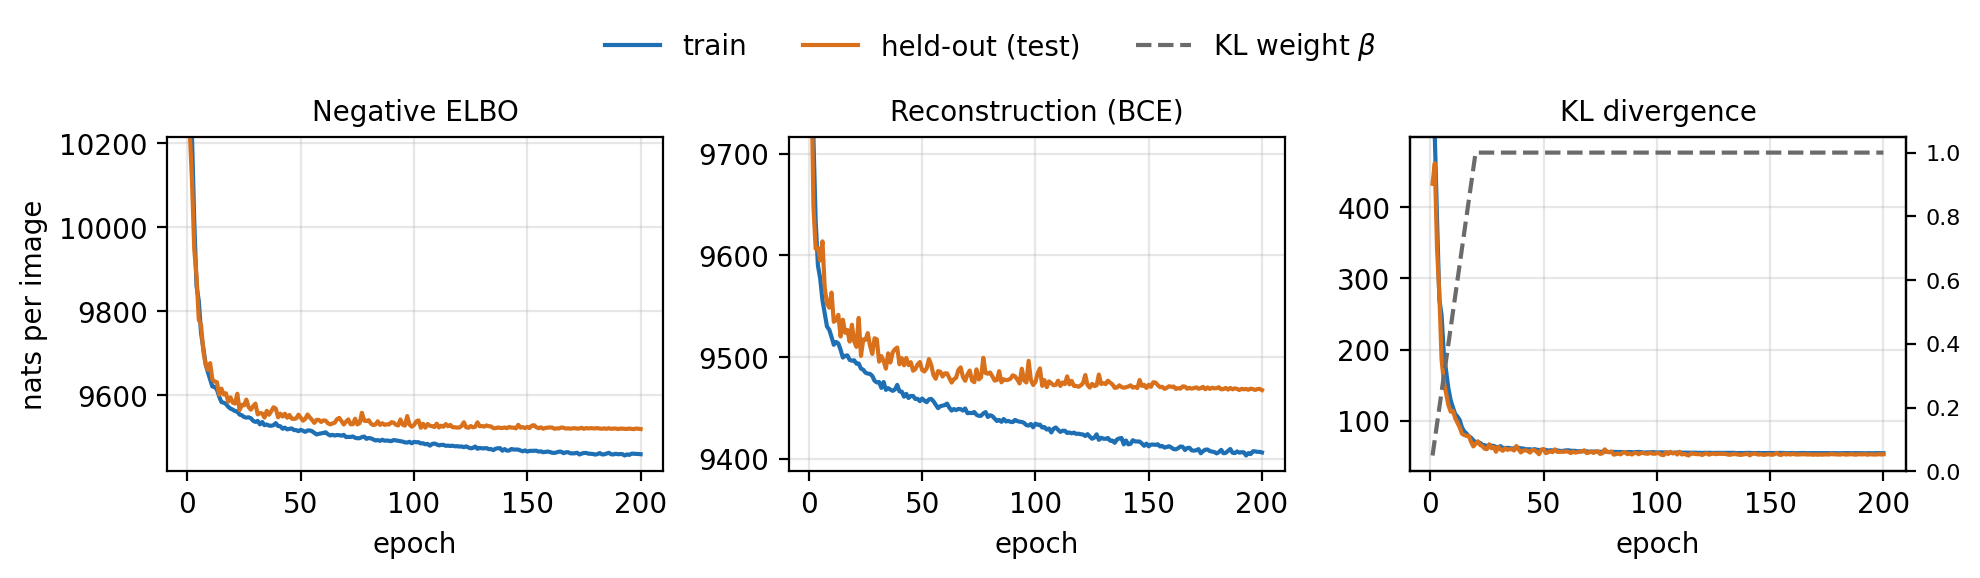
\includegraphics[width=0.88\linewidth]{loss_curves.png}
  \caption{Per-image training curves (epoch~1 is off-scale). Held-out losses
    are computed with $\beta=1$ after every epoch. The dashed line is the KL
    annealing schedule.}
  \label{fig:loss}
\end{figure}

\paragraph{Training dynamics.}
Figure~\ref{fig:loss} shows the loss curves. While $\beta$ is small the KL term
starts high and then drops quickly as $\beta$ rises. It
settles at ${\approx}53$\,nats per image without collapsing, so the latent
code stays informative. The final negative ELBO is 9{,}460 nats on train
and 9{,}520 on held-out data. The held-out reconstruction term flattens
after about 120 epochs while the training term keeps falling, a mild overfit
of ${\approx}0.6\%$. The held-out loss never rises (its minimum is at epoch
197), so we keep the final checkpoint.

\begin{figure}[!b]
  \centering
  \begin{subfigure}[b]{\linewidth}
    \centering
    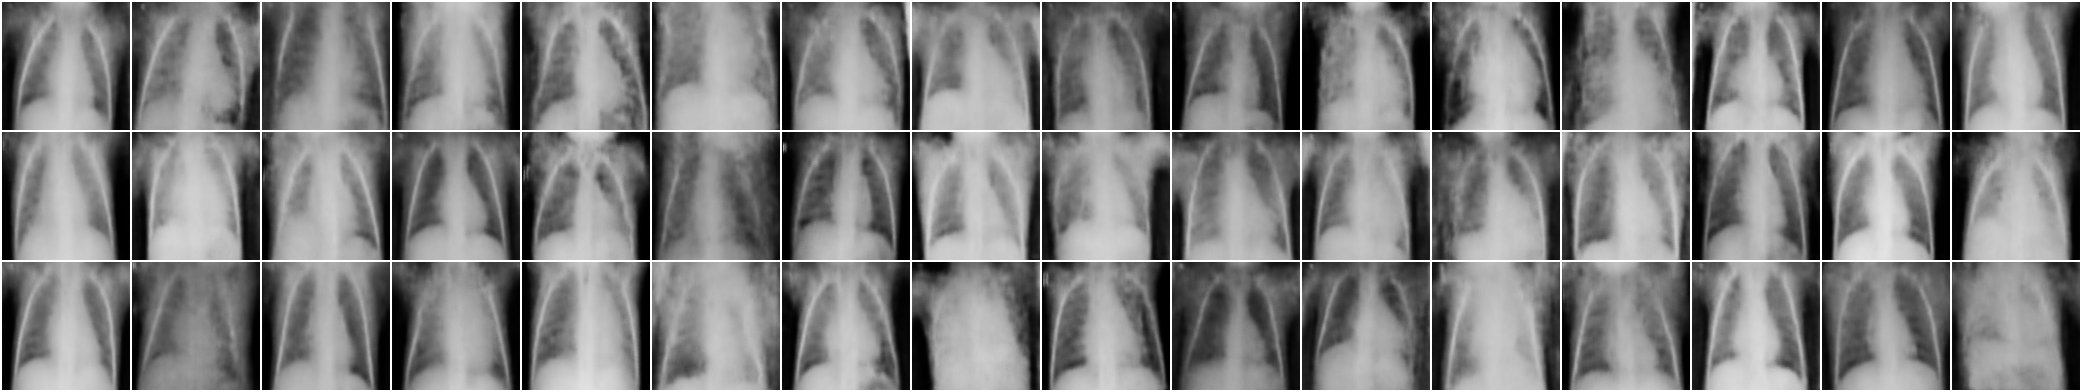
\includegraphics[width=\linewidth]{generated_samples.png}
    \caption{48 random samples decoded from $\vect{z}\sim\mathcal{N}(\vect{0},\vect{I})$.}
    \label{fig:samples}
  \end{subfigure}\\[0.4em]
  \begin{subfigure}[b]{\linewidth}
    \centering
    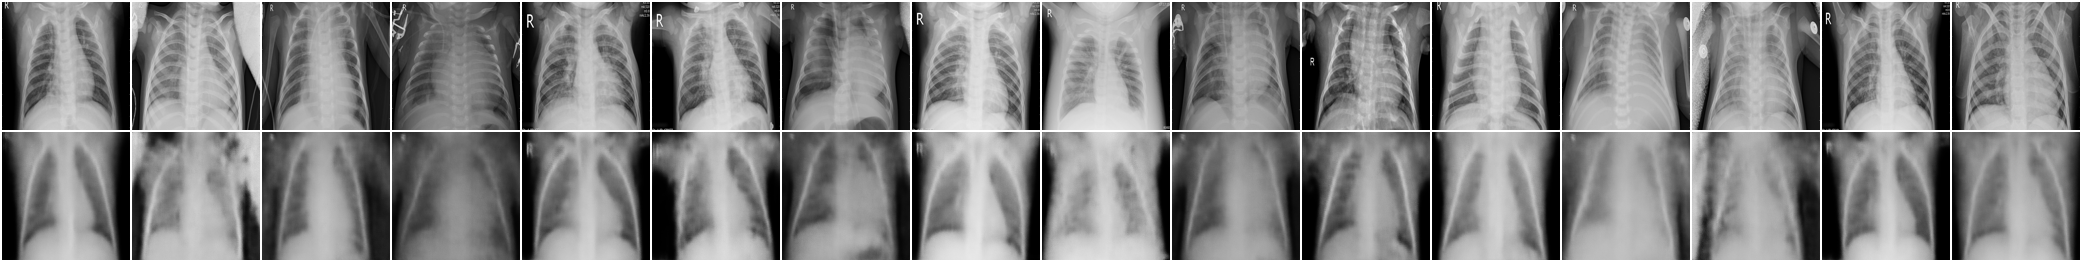
\includegraphics[width=\linewidth]{reconstructions.png}
    \caption{Held-out test originals (top) and their reconstructions from the posterior mean (bottom).}
    \label{fig:recon}
  \end{subfigure}
  \caption{Generated and reconstructed chest X-rays ($128\times128$).}
  \label{fig:images}
\end{figure}

\paragraph{Generated images.}
The samples in Figure~\ref{fig:samples} show the key anatomy: clavicles, a rib
cage that narrows toward the apices, the cardiac silhouette and mediastinum,
the diaphragm domes and the dark film border. They also reproduce the class's variety: patchy and diffuse
airspace opacities of different severity, sometimes one-sided, together
with rotated or narrow (paediatric) chests. Reconstructions
(Figure~\ref{fig:recon}) keep pose and lung opacity but lose fine rib
edges, text and devices.

\paragraph{Sample quality.}
VAE samples reach an FID of $0.163$ (Table~\ref{tab:metrics}) versus $0.008$ for real
training images, so a large gap to real data remains. The gap is mostly
due to \emph{blur}, not to a mismatch between prior and posterior:
reconstructions of real images score no better ($0.206$) than samples,
so the decoder itself cannot produce high-frequency texture. This is the
expected failure mode of a pixel-wise factorised likelihood, which
averages over the uncertain positions of fine rib and vessel edges. IS is barely informative here, because ImageNet classes do not
describe X-rays: even real test images only reach $1.96$, versus $1.74$
for samples. A perceptual or adversarial loss would be the natural next step.

\end{document}
